\clearpage
\section{Quantum Models}
\label{sec:quantum_models}

The rationale behind building a quantum version of a Game Theory and/or Statistics problem lays in bringing phenomena like quantum superposition, and entanglement into known frameworks. Converting known classical problems into quantum games is relevant to the familiarize with the potential differences these models bring.

\subsection{Quantum Roulette}
\label{subsec:quantum_roulette}

In the arbitrary $n$-State quantum roulette,\cite{Salimi2009} presented a $n$-State roulette model using permutation matrices. 

This model is interesting because in captures the usage of permutation matrices to manipulate and change the state of the system.

To verify this model with two players we developed a Matlab simulation \ref{ap:c}, that followed the steps taken in \cite{Salimi2009}.

The game in represented in a $n$-Dimensional Hilbert Space. There is a basis in the space that represents each of the equally probable entries as shown in \eqref{eq:roulette_1}. In a sense this is a generalization of a quantum coin flip that is also used in Section \ref{sec:quantum_walk_line}.
\begin{equation}
\label{eq:roulette_1}
\vert1\rangle=\left[\begin{array}{c}
1\\
0\\
0\\
\vdots\\
0
\end{array}\right],\:\vert2\rangle=\left[\begin{array}{c}
0\\
1\\
0\\
\vdots\\
0
\end{array}\right],\:\ldots,\:\vert n\rangle=\left[\begin{array}{c}
0\\
0\\
0\\
\vdots\\
1
\end{array}\right]
\end{equation}

Each state transition is obtained using a permutation matrix denoted by $P^{i}$. There are $n!$ permutation matrices, so in the particular case of having a $3$-State roulette, there are $6$ possible transition choices. The classical strategy considered will rely on choosing an arbitrary probability distribution, that verifies\eqref{eq:roulette_2}, and that maps the usage of the permutation matrices. This step will not affect the density matrix ($\rho$) of the roulette\eqref{eq:roulette_3}.

\begin{equation}
\label{eq:roulette_3}
\rho=\frac{1}{n!}\sum_{i=0}^{n!-1}P^{i}
\end{equation}

\begin{equation}
\label{eq:roulette_2}
\sum_{i=0}^{n!-1}p_{i}=1
\end{equation}

The density matrix is diagonalizable by a Discrete Fourier Transform because it is a kind of circulant matrix\cite{Davis1994}, as we can see in \eqref{eq:roulette_4}. In \eqref{eq:roulette_4} $\lambda_{k}$ are eigenvalues of $\rho$. $\lambda_{1}=1$
while $\lambda_{2}=\lambda_{3}=\lambda_{k}=\lambda_{n-1}=0$. Each column
$i$ of the Fourier matrix will represent a eigenvector $\vert\lambda_{i}\rangle$.
If we construct the diagonalizing matrix by rotating the columns of
the Fourier Matrix we can obtain the projection states as in \eqref{eq:roulette_5}.

\begin{equation}
\label{eq:roulette_4}
F^{\dagger}\rho F=\left[\begin{array}{c}
\lambda_{1}\\
0\\
0\\
\vdots\\
0
\end{array}\begin{array}{c}
0\\
\lambda_{2}\\
0\\
\vdots\\
0
\end{array}\begin{array}{c}
\ldots\\
\ldots\\
\ldots\\
\ddots\\
\ldots
\end{array}\begin{array}{c}
0\\
0\\
0\\
\vdots\\
\lambda_{n-1}
\end{array}\right]
\end{equation}



\begin{equation}
\label{eq:roulette_5}
\vert1\rangle\langle1\vert=\left[\begin{array}{c}
1\\
0\\
0\\
\vdots\\
0
\end{array}\begin{array}{c}
0\\
0\\
0\\
\vdots\\
0
\end{array}\begin{array}{c}
\ldots\\
\ldots\\
\ldots\\
\ddots\\
\ldots
\end{array}\begin{array}{c}
0\\
0\\
0\\
\vdots\\
0
\end{array}\right]=F^{\dagger}\rho F
\end{equation}


The quantum strategy advantage in this case is that the first player
will not alter the density matrix\eqref{eq:roulette_6}.

\begin{equation}
\label{eq:roulette_6}
\rho=\sum_{i=0}^{n!-1}p_{i}P^{i}\rho P^{i\dagger},\;\sum_{i=0}^{n!-1}p_{i}=1
\end{equation}

This means that if the second player knows the initial state and the first player plays with a classical strategy, thus never modifying the system density matrix, the second player will be able to manipulate the game under optimal conditions. This result is confirms the demonstration done in \cite{Meyer1999}; on Quantum Strategies, where in a classical $2$ player zero-sum game, if one player adopts a quantum strategy, she increases her chances of winning the game.

\clearpage


%\clearpage
\subsection{Ultimatum Game}
\label{subsec:ultimatumquantum}





The ultimatum game is an example of an extensive form game where two players interact in order to divide a sum of money.

A finite amount of money (or other finite resource), is given to the players, and player $1$ must propose how the money will be divided between the two players. If the second player agrees with the proposal, the resource will be split accordingly. When the player $2$ rejects the proposal, neither player will receive the money.

If we consider that we have 100 coins, the number of coins received can be considered the expected utility associated with the proposal. The first player can either present a fair division (F), where the coins are split evenly, or an unfair division (U) (defined by a parameter $\theta >50$), game tree that represents the Ultimatum Game is shown in Figure \ref{fig:ultimatum:gametree}. To each definition of $\theta$ corresponds a game.

\begin{figure}[h]
\centering 
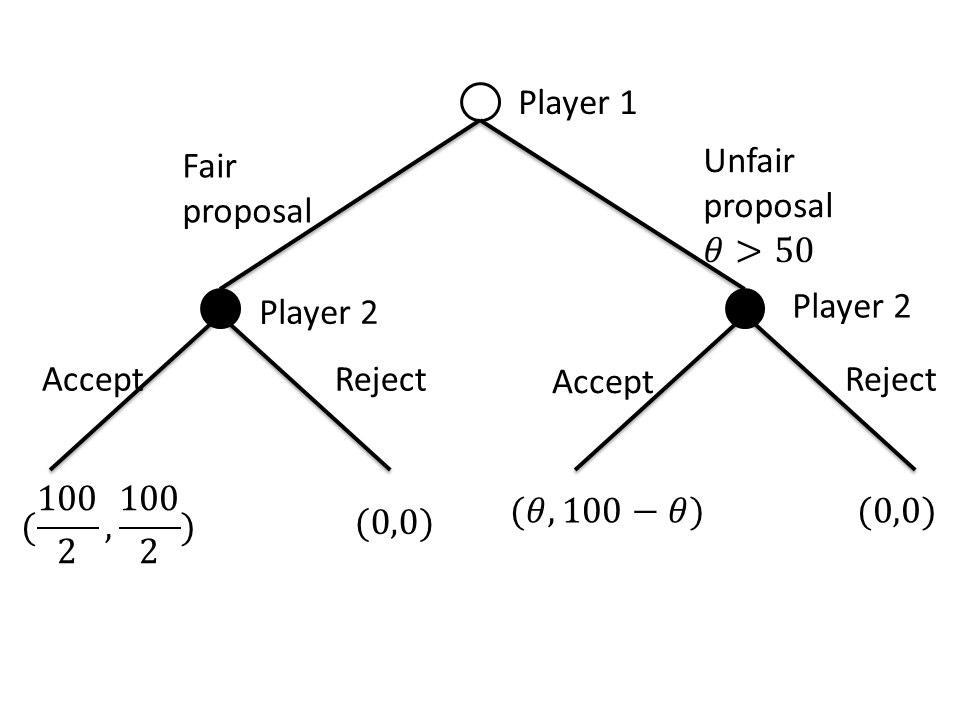
\includegraphics[scale=0.35]{Figures/ultimatum/gametree.png}
\caption{Ultimatum Game representation in the extensive form. }
\label{fig:ultimatum:gametree}
\end{figure}

\subsubsection{Quantum Model}
\label{subsec:ultimatum}

In a ``Quantum information approach to the ultimatum game''\cite{Fra2011} we are presented with a quantization scheme for the ultimatum game that uses the definition of quantum game in Section \ref{sec:background_quantum_game_theory}. 

If we present the game in Figure \ref{fig:ultimatum:gametree} in the normal form we get the matrix represented in Table \ref{tab:tabelaultimatumestoufofida}. The player $2$ has $4$ possible strategies. The strategy $A_{F}R_{U}$ means that the player $2$ will accept a fair division proposed by player $1$ but will reject a unfair division, when ($\theta > 50$).

 The quantum game representation for this game is $
\Gamma_{Ultimatum}=(\mathcal{H}^{2^{3}},\: 2,\:\vert\psi_{in}\rangle,\:\xi,\:\{\mathcal{U}_{j}\},\:\{E_{i}\})
$. The game system will consist of $3$ qubit, which correspond to the number of actions in the game. Player $1$ will be able to manipulate the qubit $1$, the player $2$ can manipulate the remaining qubits. 


\begin{center}
\begin{table}[h]
\begin{centering}
\begin{tabular}{ccccc}
\hline 
 & Player 2: $A_{F}A_{U}$ & Player 2: $A_{F}R_{U}$ & Player 2: $R_{F}A_{U}$ & Player 2: $R_{F}R_{U}$\tabularnewline
\hline 
Player 1: $F$ & $(50,50)$ & $(50,50)$& $(0,0)$ & $(0,0)$\tabularnewline
Player 1: $U$ & $(\theta,100-\theta)$ & $(0,0)$& $(\theta,100-\theta)$ & $(0,0)$\tabularnewline
\hline 
\end{tabular}
\par\end{centering}

\caption{Normal form representation of the ultimatum game.}
\label{tab:tabelaultimatumestoufofida}
\end{table}
\par\end{center}

The extensive form approach in \cite{Fra2011} allows the differentiation between simultaneous moves and sequential moves. This is accomplished by measuring the game state in order to separate game stages. This "Sequential procedure" uses the L\"{u}ders Rule, a quantum analogous of conditional probability.


The main points discussed in  \cite{Fra2011} Quantum Ultimatum approach are that the game definition presented in Section \ref{sec:background_quantum_game_theory}  makes the game more convenient to analyse than the extensive form approach.






\clearpage
\section{Overview}
\label{sec:related_work_overview}


There are more examples of games that have attracted interest in the Quantum domain. In this overview we are going to present a general picture of the work already done in this field.
 
For example various Models have been proposed to describe a quantum version of the Monty Hall problem\cite{Gill}\cite{Flitney2008}.
This popular problem\cite{Savant1990} is known for its counter-intuitiveness. The problem can be posed as a contest where the player must choose a door (from a set of $3$), and has $\frac{1}{3}$ of probability of getting a prize. After the player has chosen the door, one of the remaining $2$ doors which does not have a prize is opened. The contestant is asked whether is to her advantage to switch her initial choice.

As the host reveals information, the initial set-up is modified. This is an interesting property. Despite being a counter-intuitive problem, a quantum approach to this problem allows an in-depth comparison between the classical measurement and the quantum measurement. The classic Monty Hall problem is modelled using conditional probability and Baye's Rule to learn that it is to the advantage of the contestant to switch doors. In the quantum version, measuring the outcome of the final state yields the result, instead of taking into account the intermediate actions \cite{Fra2011}. In \cite{Gill2002} we can observe the attempt to stick as closely to the classical formulation as possible, the host has a system that is correlated to the game system.

The principal information taken from this problems is that there is not a unique way to model a classical problem\cite{Gill2002}. Therefore, when modelling a classical problem, we need to select properties that could potentially benefit from a quantum approach.

From the point of view of Quantum Cognition (a domain that seeks to introduce Quantum Mechanics Concepts in the field of Cognitive Sciences), these games are approached from the perspective of trying to model the mental state of the players in a quantum manner. The Prisoner's Dilemma is an example of a problem that has been modelled in order to explain discrepancies from the theoretical results of the classical Game Theory approach and the way humans play the game\cite{Pothos2009}. 

One last example worth mention is the quantum approach of the Stackelberg Duopoly problem\cite{Khan2011}\cite{Iqbal2008}. This is an Economics Game Theory model that seeks to represent the interactions of two companies, a market leader and a follower which play sequentially; the leader makes a decision and the follower responds. 


